\documentclass[preprint]{elsarticle}

\usepackage{hyperref}

\usepackage[english]{babel}
\usepackage[utf8]{inputenc}
\usepackage[T1]{fontenc}

\usepackage{amsmath}  % Maths
\usepackage{amsfonts} % Maths
\usepackage{amssymb}  % Maths
\usepackage{stmaryrd} % Maths (crochets doubles)

\usepackage{url}     % Mise en forme + liens pour URLs
\usepackage{array}   % Tableaux évolués

\usepackage{comment}


\usepackage{prettyref}
\newrefformat{def}{Def.~\ref{#1}}
\newrefformat{fig}{Fig.~\ref{#1}}
\newrefformat{pro}{Property~\ref{#1}}
\newrefformat{pps}{Proposition~\ref{#1}}
\newrefformat{lem}{Lemma~\ref{#1}}
\newrefformat{thm}{Theorem~\ref{#1}}
\newrefformat{sec}{Sect.~\ref{#1}}
\newrefformat{ssec}{Subsect.~\ref{#1}}
\newrefformat{suppl}{Appendix~\ref{#1}}
\newrefformat{eq}{Eq.~\eqref{#1}}
\def\pref{\prettyref}

\newdefinition{definition}{Definition}
\newdefinition{property}{Property}
\newdefinition{proposition}{Proposition}
\newdefinition{example*}{Example}
\newdefinition{example}[example*]{Example}

\usepackage{tikz}
\newdimen\pgfex
\newdimen\pgfem
\usetikzlibrary{arrows,shapes,shadows,scopes}
\usetikzlibrary{positioning}
\usetikzlibrary{matrix}
\usetikzlibrary{decorations.text}
\usetikzlibrary{decorations.pathmorphing}

% Macros relatives à la traduction de PH avec arcs neutralisants vers PH à k-priorités fixes

% Macros générales
\def\Pint{\textsc{PINT}}

% Notations générales pour PH
\newcommand{\PH}{\mathcal{PH}}
\newcommand{\PHs}{\Sigma}
\newcommand{\PHl}{L}
%\newcommand{\PHp}{\mathcal{P}}
\newcommand{\PHp}{\textcolor{red}{\mathcal{P}}}
\newcommand{\PHproc}{\mathcal{P}}
\newcommand{\PHa}{\PHh}
\newcommand{\PHh}{\mathcal{H}}
\newcommand{\PHn}{\mathcal{N}}

\newcommand{\PHhitter}{\mathsf{hitter}}
\newcommand{\PHtarget}{\mathsf{target}}
\newcommand{\PHbounce}{\mathsf{bounce}}
\newcommand{\PHsort}{\Sigma}

\def\f#1{\mathsf{#1}}
\def\focals{\f{focals}}
\def\play{\cdot}
\def\configs#1{\mathbb C_{#1\rightarrow a}}

%\newcommand{\PHfrappeR}{\textcolor{red}{\rightarrow}}
%\newcommand{\PHmonte}{\textcolor{red}{\Rsh}}

\newcommand{\PHfrappeA}{\rightarrow}
\newcommand{\PHfrappeB}{\Rsh}
%\newcommand{\PHfrappe}[3]{\mbox{$#1\PHfrappeA#2\PHfrappeB#3$}}
%\newcommand{\PHfrappebond}[2]{\mbox{$#1\PHfrappeB#2$}}
\newcommand{\PHfrappe}[3]{#1\PHfrappeA#2\PHfrappeB#3}
\newcommand{\PHfrappebond}[2]{#1\PHfrappeB#2}
\newcommand{\PHobjectif}[2]{\mbox{$#1\PHfrappeB^*\!#2$}}
\newcommand{\PHconcat}{::}
\newcommand{\PHneutralise}{\rtimes}

\def\PHget#1#2{{#1[#2]}}
%\newcommand{\PHchange}[2]{#1\langle #2 \rangle}
\newcommand{\PHchange}[2]{(#1 \Lleftarrow #2)}
\newcommand{\PHarcn}[2]{\mbox{$#1\PHneutralise#2$}}
\newcommand{\PHjoue}{\cdot}

\newcommand{\PHetat}[1]{\mbox{$\langle #1 \rangle$}}


% Notations spécifiques à ce papier
\newcommand{\PHdirectpredec}[1]{\PHs^{-1}(#1)}
\newcommand{\PHpredec}[1]{\f{pred}(#1)}
\newcommand{\PHpredecgene}[1]{\f{reg}({#1})}
\newcommand{\PHpredeccs}[1]{\PHpredec{#1} \setminus \Gamma}

\newcommand{\PHincl}[2]{#1 :: #2}

\def\ctx{\varsigma}
\def\ctxOverride{\Cap}
\def\state#1{\langle #1 \rangle}

% Notations spécifiques aux graphes d'états
%\newcommand{\PHge}{\textcolor{red}{\mathcal{GE}}}
%\newcommand{\PHt}{\mathcal{T}}
%\newcommand{\GE}{\mathcal{GE}}
%\newcommand{\GEt}{\mathcal{T}}
%\newcommand{\GEl}{\PHl}
%\newcommand{\GEa}{\PHa}
%\newcommand{\GEva}[3]{#1 \stackrel{#2}{\longrightarrow} #3}
%\newcommand{\GEval}[3]{#1 \stackrel{#2}{\Longrightarrow} #3}
%\newcommand{\GEget}[2]{\PHget{#1}{#2}}


\def\DEF{\stackrel{\Delta}=}
\def\EQDEF{\stackrel{\Delta}\Leftrightarrow}
\def\SUBSETDEF{\stackrel{\Delta}\subset}

\newcommand{\segmllabel}{\llbracket}
\newcommand{\segmrlabel}{\rrbracket}
\newcommand{\segm}[2]{\segmllabel #1 ; #2 \segmrlabel}
\newcommand{\leqsegm}{\leq_{\segmllabel\segmrlabel}}
\newcommand{\ltsegm}{<_{\llbracket\rrbracket}}

\input{macros/macros-ph}
% Macros spécifiques au Modèle de Thomas / aux RRB

\newcommand{\sN}{\mathbb{N}}

% Notations pour le modèle de Thomas (depuis thèse)
\newcommand{\GRN}{\mathcal{GRN}}
\newcommand{\IG}{\mathcal{G}}
%\def\IG{\mathrm{IG}}
\newcommand{\GRNreg}[1]{\Gamma^{-1}(#1)}
\newcommand{\GRNreslabel}{\mathsf{Res}}
\newcommand{\GRNres}[2]{\GRNreslabel_{#1}(#2)}
%\newcommand{\GRNallres}[1]{\mathsf{Res}_{#1}}
\newcommand{\GRNallres}[1]{\textcolor{red}{\mathsf{Res}_{#1}}}
\newcommand{\GRNget}[2]{\PHget{#1}{#2}}
\newcommand{\GRNstate}[1]{\PHetat{#1}}
\newcommand{\GRNstates}{\mathcal{S}}
\newcommand{\GRNedgef}[4]{#1 \xrightarrow{#2 #3} #4}
\newcommand{\GRNedge}[4]{\GRNedgef{#1}{#2,}{#3}{#4}}
\newcommand{\GRNtrans}[2]{#1 \rightarrow #2}
\newcommand{\uns}{\pm}

\def\levelsl{\mathsf{levels}}
\def\levels#1#2{\levelsl(#1\rightarrow #2)}
\def\ulevels#1#2{\overline{\levelsl}(#1\rightarrow #2)}
%\def\levelsA#1#2{\levels_+(#1\rightarrow #2)}
%\def\levelsI#1#2{\levels_-(#1\rightarrow #2)}
\def\levelsA#1#2{\textcolor{red}{\levelsl_+(#1\rightarrow #2)}}
\def\levelsI#1#2{\textcolor{red}{\levelsl_-(#1\rightarrow #2)}}
%\newcommand{\PHres}{\mathsf{Res}}

\newcommand{\Kinconnu}{\emptyset}
\newcommand{\RRGva}[3]{#1 \stackrel{#2}{\longrightarrow} #3}
\newcommand{\RRGgi}{\mathcal{G}}
\newcommand{\RRGreg}[1]{\RRGgi_{#1}}



%\definecolor{darkred}{rgb}{0.5,0,0}
%\definecolor{lightred}{rgb}{1,0.8,0.8}
%\definecolor{lightgreen}{rgb}{0.7,1,0.7}
\definecolor{darkgreen}{rgb}{0,0.5,0}
%\definecolor{darkyellow}{rgb}{0.5,0.5,0}
%\definecolor{lightyellow}{rgb}{1,1,0.6}
%\definecolor{darkcyan}{rgb}{0,0.6,0.6}
%\definecolor{darkorange}{rgb}{0.8,0.2,0}

%\definecolor{notsodarkgreen}{rgb}{0,0.7,0}

%\definecolor{coloract}{rgb}{0,1,0}
%\definecolor{colorinh}{rgb}{1,0,0}
\colorlet{coloract}{darkgreen}
\colorlet{colorinh}{red}
%\colorlet{coloractgray}{lightgreen}
%\colorlet{colorinhgray}{lightred}
%\colorlet{colorinf}{darkgray}
%\colorlet{coloractgray}{lightgreen}
%\colorlet{colorinhgray}{lightred}

%\colorlet{colorgray}{lightgray}


\tikzstyle{grn}=[every node/.style={circle,draw=black,outer sep=2pt,minimum
                size=15pt,text=black}, node distance=1.5cm]
\tikzstyle{act}=[->,draw=black,thick,color=black]
\tikzstyle{inh}=[>=|,-|,draw=black,thick, text=black,label]
%\tikzstyle{inh}=[>=|,-|,draw=colorinh,thick, text=black,label]
%\tikzstyle{act}=[->,>=triangle 60,draw=coloract,thick,color=coloract]
%\tikzstyle{inhgray}=[>=|,-|,draw=colorinhgray,thick, text=black,label]
%\tikzstyle{actgray}=[->,>=triangle 60,draw=coloractgray,thick,color=coloractgray]
\tikzstyle{inf}=[->,draw=colorinf,thick,color=colorinf]
%\tikzstyle{elabel}=[fill=none, above=-1pt, sloped,text=black, minimum size=10pt, outer sep=0, font=\scriptsize,draw=none]
\tikzstyle{elabel}=[fill=none,text=black, above=-2pt,%sloped,
minimum size=10pt, outer sep=0, font=\scriptsize, draw=none]
%\tikzstyle{elabel}=[]
\tikzstyle{sg}=[every node/.style={outer sep=2pt,minimum
                size=15pt,text=black}, node distance=2cm]



% Commandes À FAIRE
\usepackage{color} % Couleurs du texte
\newcommand{\todo}[1]{\textcolor{darkgreen}{[#1]}}


% Id est
\newcommand{\ie}{i.e. }

% Césures
\hyphenation{pa-ra-me-tri-za-tion}
\hyphenation{pa-ra-me-tri-za-tions}



\begin{document}

\begin{frontmatter}

\title{Concretizing the Process Hitting into Biological Regulatory Networks}

\author[irccyn,nii]{Maxime Folschette}
\ead{Maxime.Folschette@irccyn.ec-nantes.fr}
\author[lix]{Lo\"ic Paulev\'e}
\author[nii]{Katsumi Inoue}
\author[irccyn]{Morgan Magni}
\author[irccyn]{Olivier Roux}

\address[irccyn]{LUNAM Universit\'e, \'Ecole Centrale de Nantes, IRCCyN UMR CNRS 6597\\
(Institut de Recherche en Communications et Cybern\'etique de Nantes)\\
1 rue de la No\"e - B.P. 92101 - 44321 Nantes Cedex 3, France.}
\address[nii]{National Institute of Informatics,\\
2-1-2, Hitotsubashi, Chiyoda-ku, Tokyo 101-8430, Japan.}
\address[lix]{LIX, \'Ecole Polytechnique, 91128 Palaiseau Cedex, France.}

\begin{abstract}
\parindent 0.5cm
The Process Hitting (PH) is a recently introduced framework to model concurrent processes.
Its major originality lies in a specific restriction on the causality of actions, which
makes the formal analysis of very large systems tractable.
PH is suitable to model Biological Regulatory Networks (BRNs) with complete or partial
knowledge of cooperations between regulators by defining the most permissive dynamics
with respect to these constraints.

On the other hand, the qualitative modeling of BRNs has been widely addressed using Ren\'e Thomas'
formalism, leading to numerous theoretical work and practical tools to understand emerging behaviors.

Given a PH model of a BRN, we first tackle the inference of the underlying Interaction Graph
between components.
Then the inference of corresponding Thomas' models is provided using Answer Set Programming,
which allows notably an efficient enumeration of (possibly numerous) compatible parametrizations.

In addition to giving a formal link between different approaches for qualitative BRNs modeling, 
this work emphasizes the ability of PH to deal with large BRNs with incomplete knowledge on
cooperations, where Thomas' approach fails because of the combinatorics of parameters.
\end{abstract}

\end{frontmatter}



\section{Introduction}
As regulatory phenomena play a crucial role in biological systems, they need to be studied accurately.
Biological Regulatory Networks (BRNs) consist in sets of either positive or negative mutual effects between the components.
With the purpose of analyzing these systems, they are often modeled as graphs which make it possible to determine the possible evolutions of all the interacting components of the system.
Indeed, besides continuous models of physicists, often designed through systems of ordinary
differential equations, a discrete modeling approach was initiated by René Thomas in 1973
\cite{Thomas73}.

In this approach, the different levels of a component, such as concentration or expression levels, are abstractly represented by (positive) integer values and transitions between these levels may be considered as instantaneous.
Hence, qualitative state graphs may be derived from which we are able to formally find out all the possible behaviors expressed as sequences of transitions between these states.
Nevertheless, these dynamics can be precisely established only with regard to some discrete parameters,
hereafter called ``Thomas' parameters'',
which stand for kinds of ``focal points'', i.e. the evolutionary tendency from each state and depending on the set of the other currently interacting components.
%resources in this very state, that is, the set of the other currently interacting components.
%Hereafter, we refer to these discrete parameters as Thomas' parameters.

Thomas' modeling has motivated numerous works around the link between the Interaction Graph (IG)
(summarizing the global influences between components) and the possible dynamics (e.g.,
\cite{RiCo07,RRT08}),
model reduction (e.g., \cite{Naldi09}), formal checking of dynamics (e.g., \cite{Richard06,Naldi07}), 
and the incorporation of time (e.g., \cite{Siebert06,Ahmad08}) and probability
(e.g., \cite{Twardziok10-CMSB}) dimensions, to name but a few.
While the formal checking of dynamical properties is often limited to small networks because of the
state graph explosion, the main drawback of this framework is the difficulty to specify Thomas'
parameters, especially for large networks.

In order to address the formal checking of dynamical properties within very large BRNs, we recently
introduced in \cite{PMR10-TCSB} a new formalism, named the \emph{``Process Hitting''} (PH), to model
concurrent systems having components with a few qualitative levels.
A PH describes, in an atomic manner, the possible evolutions of a process (representing one
component at one level) triggered by the hit of at most one other process in the system.
This framework can be seen as a special class of formalisms like Petri Nets or Communicating Finite
State Machines, where the causality between actions is restricted.
Thanks to the particular structure of interactions within a PH, very efficient static analysis
methods have been developed to over- and under-approximate reachability properties making tractable
the formal analysis of BRNs with hundreds of components \cite{PMR12-MSCS}.

PH is suitable to model BRNs with different levels of abstraction in the specification of
cooperations (associated influences) between components.
This allows to model BRNs with a partial knowledge on precise evolution functions for components
by capturing the largest (the most general) dynamics.

The objectives of the work presented in this paper are the following.
Firstly, we show that starting from one PH model, it is possible to find back the underlying IG.
We perform an exhaustive search for the possible interactions on one component from all the
others, consistently with the knowledge of the dynamics that these interactions lead to and that are
expressed in PH.
The second phase of our work concerns the Thomas' parameters inference.
It consists in determining the nesting set (possibly too large) of the parameters which necessarily
lead to the satisfaction of the known cooperating constraints.
The resulting BRN dynamics is ensured to respect the PH dynamics, \ie no spurious transitions are
made possible by the inference.
Answer Set Programming (ASP) \cite{Baral03} turns out to be effective for these enumerative searches.

The outcome of this work is twofold.
The first benefit is that such an approach makes it possible to refine the construction of
BRNs with a partial and progressively brought knowledge in PH, while being able to export such
models in the Thomas' framework.
This work thus strengthens the formal link between both modelings.
The second feature of our method is that it can be applied on very large BRNs.

Finally, it must be noticed that we are not interested in this paper in the derivation of one
PH from a BRN (which was previously described in \cite{PMR10-TCSB}) but, on the contrary, to finding out
a set of BRNs from one PH.

Our work is related to the approach of \cite{Khalis09} which relies on temporal logic, and \cite{20646302,DBLP:conf/ipcat/CorblinFTCT12} which also uses constraint programming. Both aim at determining a class of models which are consistent with available partial data on the regulatory structure and dynamical properties.
%These classes are built in order to infer properties common to some studied models.
%In our approach, we intend to focus on the Thomas' parameters inference
Our method is based on a model rather than on constraints, which allows to define some properties on the system structure (such as cooperations).
Furthermore, we claim that we are able to deal with larger biological networks.

\todo{Emphasis on the new contribution since CMSB.}

\paragraph{Outline}
\pref{sec:frameworks} recalls the PH and Thomas frameworks;
\pref{sec:infer-IG} defines the IG inference from PH;
\pref{sec:infer-K} details the enumeration of Thomas parametrizations compatible with a PH
and discuss its implementation in ASP.
\pref{sec:examples} illustrates the applicability of our method on simple examples
and large biological models.

\paragraph{Notations}
$\segm{i}{j}$ is the set of integers $\{ i, i+1, \dots, j \}$.
Given an integer $k$, we note: $k < \segm{i}{j} \EQDEF k < i$ and $k > \segm{i}{j} \EQDEF k > j$.
We also define:
\begin{align*}
  \segm{i_1}{j_1} \leqsegm \segm{i_2}{j_2} &\EQDEF (i_1\leq i_2\wedge j_1\leq j_2) \enspace\text{, and:}\\
  \segm{i_1}{j_1} \ltsegm \segm{i_2}{j_2} &\EQDEF (i_1<i_2 \wedge j_1\leq j_2) \vee (i_1\leq i_2\wedge j_1 < j_2) \enspace.
\end{align*}


\section{Frameworks}\label{sec:frameworks}
\subsection{The Process Hitting framework}
\label{ssec:PH}

We recall here the definition and semantics of the Process Hitting (PH), and its usage to model
cooperation between concurrent components.
Two examples of PH modeling a BRN at different abstraction levels are given.
They serve as running examples in the rest of this article.

\medskip

A PH (\pref{def:PH}) gathers a finite number of concurrent \emph{processes}
grouped into a finite set of \emph{sorts}.
A process belongs to a unique sort and is noted $a_i$ where $a$ is the
sort and $i$ the identifier of the process within the sort $a$.
At any time, one and only one process of each sort is present; a state of the PH thus corresponds to the set of such processes.
 
The concurrent interactions between processes are defined by a set of
\emph{actions}.
Actions describe the replacement of a process by another of the same sort
conditioned by the presence of at most one other process in the current
state of the PH.
An action is denoted by $\PHfrappe{a_i}{b_j}{b_k}$ where $a_i,b_j,b_k$ are processes
of sorts $a$ and $b$.
It is required that $b_j\neq b_k$ and that $a=b\Rightarrow a_i=b_j$.
An action $h=\PHfrappe{a_i}{b_j}{b_k}$ is read as ``$a_i$ \emph{hits} $b_j$ to
make it bounce to $b_k$'', and
$a_i,b_j,b_k$ are called respectively \emph{hitter}, \emph{target} and
\emph{bounce} of the action, and can be referred to as
$\PHhitter(h), \PHtarget(h), \PHbounce(h)$, respectively.

\begin{definition}[Process Hitting]\label{def:PH}
A \emph{Process Hitting} is a triple $(\PHs,\PHl,\PHa)$:
\begin{itemize}
\item $\PHs \DEF \{a,b,\dots\}$ is the finite set of \emph{sorts};
\item $\PHl \DEF \prod_{a\in\PHs} \PHl_a$ is the set of states with $\PHl_a = \{a_0,\dots,a_{l_a}\}$
the finite set of \emph{processes} of sort $a\in\Sigma$ and $l_a$ a positive integer with
	$a\neq b\Rightarrow \forall(a_i,b_j)\in\PHl_a\times\PHl_b,a_i\neq b_j$;
\item $\PHa \DEF \{ \PHfrappe{a_i}{b_j}{b_k}, \ldots \mid
					(a,b)\in\PHs^2 \wedge (a_i,b_j,b_k)\in \PHl_a\times\PHl_b\times\PHl_b$ \\
	\hspace*{2cm} $\wedge b_j\neq b_k \wedge a=b\Rightarrow a_i=b_j\}$
			is the finite set of \emph{actions}.
\end{itemize}
$\PHproc$ denotes the set of all processes ($\PHproc \DEF \{ a_i\mid a\in\PHs \wedge a_i\in\PHl_a\}$).
\end{definition}

\noindent
The sort of a process $a_i$ is referred to as $\PHsort(a_i)=a$ and the set of
sorts present in an action $h\in\PHa$ as 
$\PHsort(h) = \{\PHsort(\PHhitter(h)),\PHsort(\PHtarget(h))\}$.
Given a state $s\in \PHl$, the process of sort $a\in\PHs$ present in $s$ is
denoted by $\PHget{s}{a}$, that is the $a$-coordinate of the state $s$.
If $a_i\in \PHl_a$, we define the notation $a_i\in s \EQDEF \PHget{s}{a}=a_i$.

An action $h=\PHfrappe{a_i}{b_j}{b_k} \in\PHa$ is \emph{playable} in $s\in L$
if and only if $\PHget{s}{a}=a_i$ and $\PHget{s}{b}=b_j$.
In such a case, $(s\play h)$ stands for the state resulting from the play of
the action $h$ in $s$, that is 
$\PHget{(s\play h)}{b} = b_k$ and 
$\forall c\in\PHs, c\neq b, \PHget{(s\play h)}{c} = \PHget{s}{c}$.
For the sake of clarity, $((s\play h)\play h')$, $h'\in\PHa$ is abbreviated as
$(s\play h\play h')$.

\begin{example}
\pref{fig:runningPH-1} represents a PH $(\PHs,\PHl,\PHa)$ with
$\PHs = \{a,b,c\}$,
$\PHl_a = \{a_0,a_1,a_2\}$,
$\PHl_b = \{b_0, b_1\}$,
$\PHl_c = \{c_0, c_1\}$, and
\begin{align*}
\PHa & = \{
	\PHfrappe{a_2}{b_1}{b_0},
&&  \PHfrappe{b_0}{a_2}{a_1},
&&	\PHfrappe{c_0}{a_2}{a_1},\\
&&& \PHfrappe{b_0}{a_1}{a_0},
&&	\PHfrappe{c_0}{a_1}{a_0},\\
&&& \PHfrappe{b_1}{a_0}{a_1},
&&	\PHfrappe{c_1}{a_0}{a_1},\\
&&& \PHfrappe{b_1}{a_1}{a_2},
&&	\PHfrappe{c_1}{a_1}{a_2} \}\enspace.
\end{align*}
The action $h=\PHfrappe{b_1}{a_1}{a_2}$ is playable in the state
$s = \state{b_1,a_1,c_0}$; and $s\play h=\state{b_1,a_2,c_0}$.

\begin{figure}[t]
\centering
\scalebox{1.3}{
\begin{tikzpicture}
\TSort{(0,0)}{a}{3}{r}
\TSort{(-3,0.5)}{b}{2}{l}
\TSort{(3,0.5)}{c}{2}{r}

\THit{b_1}{very thick}{a_0}{.west}{a_1}
\THit{b_1}{very thick}{a_1}{.north west}{a_2}
\THit{b_0}{}{a_2}{.west}{a_1}
\THit{b_0}{}{a_1}{.west}{a_0}

\path[bounce, bend left=60]
\TBounce{a_1}{very thick}{a_2}{.south}
\TBounce{a_0}{very thick}{a_1}{.south}
;
\path[bounce, bend right=60]
\TBounce{a_2}{}{a_1}{.north}
\TBounce{a_1}{}{a_0}{.north}
;

\THit{c_1}{very thick}{a_0}{.east}{a_1}
\THit{c_1}{very thick}{a_1}{.north east}{a_2}
\THit{c_0}{}{a_2}{.east}{a_1}
\THit{c_0}{}{a_1}{.east}{a_0}

\path[bounce, bend right=60]
\TBounce{a_1}{very thick}{a_2}{.south east}
\TBounce{a_0}{very thick}{a_1}{.south east}
;
\path[bounce, bend left=60]
\TBounce{a_2}{}{a_1}{.north}
\TBounce{a_1}{}{a_0}{.north east}
;

\THit{a_2}{bend right}{b_1}{.north east}{b_0}
\path[bounce, bend left=80]
\TBounce{b_1}{out=100,in=140}{b_0}{.north}
;

\end{tikzpicture}
}
\caption{\label{fig:runningPH-1}
A Process Hitting (PH) example.
Sorts are represented by labeled boxes, and processes by circles (ticks are
the identifiers of the processes within the sort, for instance, $a_0$ is the
process ticked $0$ in the box $a$).
An action (for instance $\PHfrappe{b_1}{a_1}{a_2}$) is represented by a pair of
directed arcs, having the hit part ($b_1$ to $a_1$) in plain line and the bounce
part ($a_1$ to $a_2$) in dotted line.
Here, actions involving $b_1$ or $c_1$ are in thick lines.
%The current state is represented by the grayed processes:
%$\state{a_0,b_1,c_0,d_0}$.
}
\end{figure}

This PH example actually models a BRN where the component $a$ has three qualitative
levels and components $b$ and $c$ are boolean.
In this BRN, $b$ and $c$ activate $a$, while $a$ inhibits $b$.
The inhibition of $b$ by $a$ is only effective when $a$ is at level $2$ (noted: $a_2$);
in the other cases, $b$ cannot evolve in any direction.
The activation of $a$ by $b$ ($c$) is encoded by the actions making the level of $a$ increase (resp.
decrease) when $b$ ($c$) is present (resp. absent).
It is worth noticing that the activation of $a$ by $b$ ($c$) is independent from $c$ ($b$).
This may express a lack of knowledge on the cooperation between these two regulators:
we thus model an over-approximation of the possible actions.
\end{example}

\paragraph{Modeling cooperation}
As described in \cite{PMR10-TCSB}, the cooperation between several processes to make another process bounce can be
expressed in PH by building a \emph{cooperative sort}.
\pref{fig:PH-cooperativity} shows an example of cooperation between processes $b_1$ and $c_1$ to
make $a_1$ bounce to $a_2$:
a cooperative sort $bc$ is defined with 4 processes (one for each sub-state of the presence of
processes $b_1$ and $c_1$).
For the sake of clarity, the processes of $bc$ are indexed using the sub-state they represent.
Hence, $bc_{01}$ represents the sub-state $\state{b_0,c_1}$, and so on.
Each process of sort $b$ and $c$ hit $bc$ to make it bounce to the process reflecting the status of the sorts $b$
and $c$ (e.g., $\PHfrappe{b_1}{bc_{00}}{bc_{10}}$ and $\PHfrappe{b_1}{bc_{01}}{bc_{11}}$).
Then, it is process $bc_{11}$ which hits $a_1$ to make it bounce to $a_2$ instead of
independent hits from $b_1$ and $c_1$.

\begin{figure}[p]
\centering
\scalebox{1.3}{
\begin{tikzpicture}
\TSort{(0,0)}{b}{2}{t}
\TSort{(0,-3.8)}{c}{2}{b}
\TSort{(4.5,-3)}{a}{3}{r}

\TSetTick{bc}{0}{00}
\TSetTick{bc}{1}{01}
\TSetTick{bc}{2}{10}
\TSetTick{bc}{3}{11}
% \TSetSortLbcel{bc}{$\neg a\wedge b$}
\TSort{(-0.5,-2)}{bc}{4}{b}

\THit{b_1}{very thick,bend right}{bc_0}{.north}{bc_2}
\THit{b_1}{very thick,bend right}{bc_1}{.north}{bc_3}
\THit{b_0}{}{bc_2}{.north west}{bc_0}
\THit{b_0}{}{bc_3}{.north west}{bc_1}

\THit{c_0}{}{bc_1}{.south}{bc_0}
\THit{c_0}{}{bc_3}{.south}{bc_2}
\THit{c_1}{very thick}{bc_0}{.south}{bc_1}
\THit{c_1}{very thick}{bc_2}{.south}{bc_3}

\path[bounce, bend right=25]
\TBounce{bc_2}{}{bc_0}{.north east}
\TBounce{bc_3}{}{bc_1}{.north east}
;
\path[bounce, bend left=80, distance=30]
\TBounce{bc_0}{very thick}{bc_2}{.north}
\TBounce{bc_1}{very thick}{bc_3}{.north}
;
\path[bounce, bend right]
\TBounce{bc_0}{very thick}{bc_1}{.west}
\TBounce{bc_2}{very thick}{bc_3}{.west}
;
\path[bounce, bend left]
\TBounce{bc_3}{}{bc_2}{.east}
\TBounce{bc_1}{}{bc_0}{.east}
;

\THit{bc_3}{}{a_1}{.west}{a_2}
\path[bounce, bend left=40]
\TBounce{a_1}{}{a_2}{.south west}
;

\end{tikzpicture}
}

\caption{\label{fig:PH-cooperativity}
A PH modeling a cooperativity between $b_1$ and $c_1$ to make
$a_1$ bounce to $a_2$.
Actions involving $b_1$ or $c_1$ are in thick lines.
}
\end{figure}
\begin{figure}[p]
\centering
\scalebox{1.3}{
\begin{tikzpicture}
\path[use as bounding box] (-4,-1.9) rectangle (4.5,3.9);

\TSort{(0,0)}{a}{3}{l}
\TSort{(3, 3)}{b}{2}{t}
\TSort{(3,-1)}{c}{2}{b}

\TSetTick{bc}{0}{00}
\TSetTick{bc}{1}{01}
\TSetTick{bc}{2}{10}
\TSetTick{bc}{3}{11}
% \TSetSortLbcel{bc}{$\neg a\wedge b$}
\TSort{(-3,-0.5)}{bc}{4}{l}

\THit{bc_3}{}{a_1}{.north west}{a_2}
\THit{bc_0}{}{a_1}{.south west}{a_0}
\path[bounce]
\TBounce{a_1}{bend left}{a_2}{.south west}
\TBounce{a_1}{bend right}{a_0}{.north west}
;

\THit{b_0}{}{a_2}{.east}{a_1}
\THit{b_1}{}{a_0}{.north east}{a_1}
\path[bounce]
\TBounce{a_2}{bend left}{a_1}{.north east}
\TBounce{a_0}{bend right=20}{a_1}{.south}
;

\THit{c_0}{bend right}{a_2}{.south east}{a_1}
\THit{c_1}{bend right}{a_0}{.east}{a_1}
\path[bounce]
\TBounce{a_2}{bend left=20}{a_1}{.north}
\TBounce{a_0}{bend right=30}{a_1}{.south east}
;

\path[dashed,hit]
	(2,-1.3) edge[bend left=10] (-2.3,-0.7)
	(2.2, 3.3) edge[bend right=10] (-2.3,3)
;

\THit{a_2}{bend left,out=40,in=80}{b_1}{.north west}{b_0}
\path[bounce, bend right]
\TBounce{b_1}{}{b_0}{.east}
;

\end{tikzpicture}
}

\caption{\label{fig:runningPH-2}
PH resulting from the refinement of the one in \pref{fig:runningPH-1} by the
specification of several cooperations.
The actions from $b$ and $c$ to the cooperative sort $bc$ are identical to those defined in
\pref{fig:PH-cooperativity} and are represented here by a single dashed arc.
}
\end{figure}

We note that cooperative sorts are standard PH sorts and do not involve any
special treatment regarding the semantics of related actions.

When the number of cooperating processes is large, it is possible to chain several cooperative sorts
to prevent the combinatoric explosion of the number of processes created within cooperative sorts.
For instance, if $b_1$, $c_1$, and $d_1$ cooperate, one can create a cooperative sort $bc$ with 4
processes reflecting the presence of $b_1$ and $c_1$, and a cooperative sort $bcd$ with 4 processes
reflecting the presence of $bc_{11}$ and $d_1$.  Such constructions are helpful in PH
as the static analysis of dynamics developed in \cite{PMR12-MSCS} does not suffer from the number of
sorts, but on the number of processes within a single sort.

While the construction of cooperation in PH allows to encode any boolean functions
between cooperating processes \cite{PMR10-TCSB}, it is worth noticing they introduce a temporal
shift in their application.
This allows the existence of interleaving of actions leading to a cooperative sort representing a
past sub-state of the presence of the cooperative processes.
The resulting behavior is then an over-approximation
of the realization of an instantaneous cooperation.
However, it is possible to obtain the exact behavior of the cooperations by using the semantics with prioritized actions defined in~\cite{FPMR13-CS2Bio}.
Although this new semantics is not further described here, the inferences given in \pref{sec:infer-IG} \& \ref{sec:infer-K} do ignore the temporal shift induced by the cooperative sorts.

\begin{example}
The PH in \pref{fig:runningPH-2} results from the refinement of the PH in \pref{fig:runningPH-1}
where several cooperations have been specified.
In particular, the bounce to $a_2$ is the result of a cooperation between $b_1$ and $c_1$; and the
bounce to $a_0$ of a cooperation between $b_0$ and $c_0$.
Hence, this PH expresses a BRN where $a$ requires both $b$ and $c$ active to reach its
highest level, and $a$ does not become inactive unless both $b$ and $c$ are inactive.
\end{example}

\subsection{Thomas' modeling}

We concisely present Thomas' modeling of BRNs dynamics, merely inspired by
\cite{Richard06,BernotSemBRN}.
In order to enlarge the class of Thomas' models compatible with PH dynamics (w.r.t. the presented
inference),
we propose the notion of unsigned edge modeling an interaction whose nature (activation or inhibition) is undefined,
and we extend the classical parametrization formalism by setting parameters to intervals of values instead of single values.
We briefly discuss these additions.

Thomas' formalism lies on two complementary descriptions of the system. First, the
\emph{Interaction Graph} (IG) models the structure of the system by defining the components'
mutual influences and the conditions of these influences.
The \emph{parametrization} then specifies the levels towards which tends a component when a given
configuration of its regulators applies.

The IG is composed of nodes that represent components, and edges labeled with a threshold that stand
for either positive or negative regulations (\pref{def:ig}).
For such a regulation to take place, the expression level of its head component has to be higher than its threshold; otherwise, the opposite influence is expressed.
The uniqueness of these regulations makes the following sections simpler.
%Therefore, for any component $b$, a predecessor $a$ of $b$ such that we have $a \xrightarrow{t} b$
%can be either an activator or an inhibitor of $a$, according to the sign of the interaction and if the expression level of $b$ if above or below the threshold $t$.
%We call $\levelsA{a}{b}$ (resp. $\levelsI{a}{b}$) the levels of $a$ where it is an
%activator (resp. inhibitor) of $b$ (\pref{def:levels});
We call $\levels{a}{b}$ the levels of $a$ above the threshold of $\GRNedge{a}{s}{t}{b}$;
$l_a$ denotes the maximum level of $a$.
%For the sake of simplicity and to establish a parallel with PH, if $a$ represents a component, we call $a_i$ its $i^\text{th}$ expression level.
\rewrite{Rewrite + reference + add some glue}
%\new{Added unsigned edges ($\uns$) that stand for an unknown king of regulation.
%The definition of $\levels{a}{b}$ now gives the levels for which $a$ regulates $b$ (i.e. $a > t$), independently from the regulation sign.}

\begin{definition}[Interaction Graph]
\label{def:ig}
%An \emph{Interaction Graph} (IG) is a quadruplet $(\Gamma, E_+, E_-, E_\uns)$ where $\Gamma$ is a finite number of \emph{components},
%and $E_+$ (resp. $E_-$) $\subset \{a \xrightarrow{t} b \mid a, b \in \Gamma \wedge t \in [1; l_a]\}$
%is the set of positive (resp. negative) \emph{regulations} between two nodes, labeled with a \emph{threshold}.
An \emph{Interaction Graph} (IG) is a couple $(\Gamma, E)$ where $\Gamma$ is the finite set of \emph{components},
and $E$
%and $E_+$ (resp. $E_-$) $\subset \{a \xrightarrow{t} b \mid a, b \in \Gamma \wedge t \in [1; l_a]\}$
is the finite set of 
%positive (resp. negative)
\emph{regulations} between two nodes, labeled with a \emph{sign} and a \emph{threshold}:
$$E \DEF \{ \GRNedge{a}{s}{t}{b}, \ldots \mid a, b \in \Gamma \wedge s \in \{ +, -, \uns \} \wedge t \in [1; l_a]\}$$
A regulation from $a$ to $b$ is uniquely referenced:
$$\forall \GRNedge{a}{s}{t}{b} \in E, \forall \GRNedge{a}{s'}{t'}{b} \in E, s = s' \wedge t = t' \enspace.$$
%if $a \xrightarrow{t} b \in E_+$ (resp. $E_-$),
%$\nexists a \xrightarrow{t'} b \in E_+ \text{ (resp. $E_-$)}, t' \neq t$
%and $\nexists a \xrightarrow{t'} b \in E_-\text{ (resp. $E_+$)}, t' \in \mathbb{N}$.
\end{definition}

Given this definition, we denote as a shortcut:
$E_s \DEF \{ \GRNedge{a}{s}{t}{b} \in E \}$
for $s \in \{ +, -, \uns \}$.
Furthermore, for all component $a \in \Gamma$, 
we denote $\GRNreg{a}$ the set of its regulators as defined in \pref{eq:grn-regulators}.
\[
  \label{eq:grn-regulators}
  \GRNreg{a} \DEF \{ b\in\Gamma\mid \exists \GRNedge{b}{s}{t}{a} \in E \}
\]
The maximum level $l_a$ of a component $a$ is usually chosen equal to the number of outgoing edges of $a$, \ie the number of components that $a$ regulates.
Indeed, each discrete expression level in $[0 ; l_a]$ stands for an arbitrary set of concentration levels for which $a$ has a certain influence on several other components it regulates.
Allowing more expression levels makes several levels useless as they represent the same influence of $a$ than some other levels;
on the contrary, reducing the maximum level requires that several thresholds on outgoing edges of $a$ share the same value, which is biologically unlikely.
However, these considerations are usually taken into account when one has to directly build a model in this framework, but are not mandatory.
In the scope of this paper, we allow any number of levels for components, without considering the number of outgoing edges,
as the number of processes in a PH sort is not constrained in any way.


%$E_+(a) = \{b \in \Gamma \mid \exists b \xrightarrow{t} a \in
%E_+\}$ (resp. $E_-(a) = \{b \in \Gamma \mid \exists b \xrightarrow{t} a \in E_-\}$) denotes the set
%of its positive (resp. negative) regulators; and
%$\GRNreg{a} = E_+(a)\cup E_-(a)$ the set of its regulators.

\begin{definition}[Effective levels ($\levelsl$)]\label{def:levels}
%Let $(\Gamma,E)$ be an IG and $a, b \in \Gamma$ two of its components.
Let $b \in \Gamma$ and $a \in \GRNreg{a}$;
we define: $\levels{a}{b} \DEF [t; l_a]$ and $\ulevels{a}{b} \DEF [0; t-1]$.
%%%
%\begin{itemize}
%  \item if $a \xrightarrow{t} b \in E_+$, $\levelsA{a}{b} \DEF [t; l_a]$ and
%    $\levelsI{a}{b} \DEF [0; t-1]$;
%  \item if $a \xrightarrow{t} b \in E_-$, $\levelsA{a}{b} \DEF [0; t-1]$ and
%    $\levelsI{a}{b} \DEF [t; l_a]$;
%  \item otherwise, $\levelsA{a}{b} \DEF \levelsI{a}{b} \DEF \emptyset$.
%%%
%  \item if $\GRNedge{a}{s}{t}{b} \in E$, $\levels{a}{b} \DEF [t; l_a]$;
%  \item otherwise, $\levels{a}{b} \DEF \emptyset$.
%\end{itemize}
\end{definition}

\begin{example*}
\pref{fig:runningBRN}(left) represents an Interaction Graph $(\Gamma,E)$ with
$\Gamma = \{a, b, c\}$ and:
\begin{align*}
  E_+ &= \{\GRNedgef{b}{+}{1}{a}, \GRNedgef{c}{+}{1}{a}\} &
  E_\uns &= \emptyset \\
  E_- &= \{\GRNedgef{a}{-}{2}{b}\}
\end{align*}
Hence:
\begin{align*}
  \GRNreg{a} &= \{ b, c \} &
  \GRNreg{b} &= \{ a \} \\
  \GRNreg{c} &= \emptyset
\end{align*}
%This IG can represent the same behavior as the PH given in \pref{fig:runningPH-2}.
\end{example*}

\begin{figure}[t]
\begin{minipage}{0.4\linewidth}
\centering
\scalebox{1.2}{
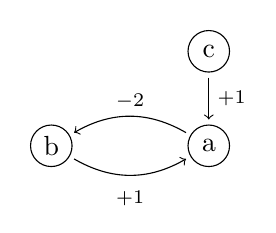
\begin{tikzpicture}[grn]
\path[use as bounding box] (-0.3,-0.75) rectangle (2.5,1.5);
\node[inner sep=0] (a) at (2,0) {a};
\node[inner sep=0] (b) at (0,0) {b};
\node[inner sep=0] (c) at (2,1.2) {c};
%\path
%  node[elabel, below=-1em of a] {$0..2$}
%  node[elabel, below=-1em of b] {$0..1$}
%  node[elabel, below=-1em of c] {$0..1$};
\path[->]
  (b) edge[bend right] node[elabel, below=-2pt] {$+1$} (a)
  (c) edge node[elabel, right=-2pt] {$+1$} (a)
  (a) edge[bend right] node[elabel, above=-5pt] {$-2$} (b);
\end{tikzpicture}
}
\end{minipage}
\begin{minipage}{0.6\linewidth}
\centering
\begin{align*}
K_{a,\{b,c\}} &= [2 ; 2] & K_{b,\emptyset} &= [0 ; 1] \\
K_{a,\{b\}} &= [1 ; 1] & K_{b,\{a\}} &= [0 ; 0] \\
K_{a,\{c\}} &= [1 ; 1] &&\\
K_{a,\emptyset} &= [0 ; 0] & K_{c,\emptyset} &= [0 ; 1]
\end{align*}
\end{minipage}
\caption{\label{fig:runningBRN}
(left)
IG example.
%Components are represented by nodes labeled with a name and possible expression levels.
Regulations are represented by the edges labeled with their sign and threshold.
For instance, the edge from $b$ to $a$ is labeled $+1$, which stands for: $\GRNedgef{b}{+}{1}{a}$.
%and means that if the level of expression of $b$ is equal to (i.e. above) 1, then $b$ activates $a$,
%otherwise, $b$ inhibits $a$.
(right)
Example parametrization of the left IG.
}
\end{figure}

A \emph{state} $s$ of an IG $(\Gamma, E)$ is an element in $\GRNstates \DEF \prod_{a \in \Gamma} [0;l_a]$.
$\GRNget{s}{a}$ refers to the level of component $a$ in $s$.
\rewrite{Functional definition of a state? (More rigorous)}
The specificity of Thomas' approach lies in the use of discrete \emph{parameters} to represent the
focal level interval towards which the component will evolve in each configuration of its regulators
(\pref{def:param}).
Indeed, for each possible state of a BRN, all regulators of a component $a$ can be divided into
\emph{activators} and \emph{inhibitors}, given their type of interaction and expression level,
referred to as the \emph{resources} of $a$ in this state (\pref{def:resources}).
%
%\new{No more $A,B$ but sets $\omega$ of resources instead. Definitions of $K$ were adapted.}

\begin{definition}[Resources ($\GRNreslabel$)]\label{def:resources}
For a given component $a \in \Gamma$ and a state $s \in \GRNstates$,
the set of regulators of $a$ whose level in $s$ is above the required threshold to regulate $a$
is called the set of \emph{resources} of $a$ in $s$ and is noted $\GRNres{a}{s}$:
%\begin{align*}
%  A &= \{b \in \Gamma \mid \GRNget{s}{b} \in \levelsA{b}{a}\} \\
%  B &= \{b \in \Gamma \mid \GRNget{s}{b} \in \levelsI{b}{a}\}
%\end{align*}
$$\GRNres{a}{s} \DEF \{ b \in \GRNreg{a} \mid \GRNget{s}{b} \in \levels{b}{a} \}$$
%We also denote: $\GRNallres{a} = \{(A;B) \mid \exists s \in \textstyle\prod_{a \in \Gamma} [0;l_a], \GRNres{a}{s} = A,B\}$
%We also denote: $\GRNallres{a} = \{ \omega \subset \GRNreg{a} \}$
\end{definition}

\begin{definition}[Discrete parameter $K_{a,\omega}$ and Parametrization $K$]\label{def:param}
For a given component $a \in \Gamma$ and $\omega \subset \GRNreg{a}$ a set of regulators of $a$,
the discrete \emph{parameter} $K_{a,\omega} = [i; j]$ is a non-empty interval towards which $a$ will tend
in the states where its resources are exactly the regulators in $\omega$.
The complete map $K$ of discrete parameters for $\IG$ is called a \emph{parametrization} of $\IG$.
%For a given component $a \in \Gamma$ and $A$ (resp. $B$) $\subset \GRNreg{a}$ a set of its activators (resp. inhibitors) such that $A \cup B = \GRNreg{a}$ and $A \cap B = \emptyset$,
%the discrete \emph{parameter} $K_{a,A,B} = [i; j]$ is a non-empty interval towards which $a$ will tend
%in the states where its activators (resp. inhibitors) are the regulators in set $A$ (resp. $B$).
%The complete map $K$ of discrete parameters for $\IG$ is called a \emph{parametrization} of $\IG$.
\end{definition}
%A consequence of this definition is that $0 \leq i_1 \leq i_2 \leq l_a$.
%We also denote: $j < K_{a,A,B} \Leftrightarrow j < i_1$ and $j > K_{a,A,B} \Leftrightarrow j> i_2$.

%\begin{example*}
%\pref{fig:runningBRN}(right) gives a Parametrization of the IG of \pref{fig:runningBRN}(left).
%\end{example*}

At last, \pref{def:dynamics} gives the asynchronous dynamics of a BRN using Thomas' parameters.
From a given state $s$, a transition to another state $s'$ is possible provided that only one component $a$ will evolve of one level towards $K_{a,\GRNres{a}{s}}$,
as stated by the definition of the transition relation $\GRNtrans{s}{s'}$.
%
%\new{Use a transition relation instead of an indeterministic function.}

\begin{definition}[Asynchronous dynamics ($\GRNtrans{}{}$)]\label{def:dynamics}
The dynamics of a BRN using Thomas' parameters is given by the transition relation $\GRNtrans{}{} \in \GRNstates \times \GRNstates$ defined by:
\begin{align*}
  \forall s, s' \in \GRNstates, \GRNtrans{s}{s'} &\Longleftrightarrow \exists a \in \Gamma, \GRNget{s}{a} \notin K_{a, \GRNres{a}{s}} \wedge \GRNget{s'}{a} = \GRNget{s}{a} + f^a(s) \\
    & \qquad \wedge \forall b \in \Gamma, b \neq a \Rightarrow \GRNget{s}{b} = \GRNget{s'}{b}
\end{align*}
with: $f^a(s) = 
  \begin{cases}
    +1 & \text{if } \GRNget{s}{a} < K_{a, \GRNres{a}{s}} \\
    -1 & \text{if } \GRNget{s}{a} > K_{a, \GRNres{a}{s}} \\
  \end{cases}$
\begin{comment}
Let $s$ be a state of a BRN using Thomas' parameters $(\IG, K)$ where $\IG = (\Gamma, E_+, E_-)$.
The state that succeeds to $s$ is given by the indeterministic function $f(s)$:
\begin{align*}
  f(s)  & = s' \Leftrightarrow \exists a \in \Gamma,
    \GRNget{s'}{a} = f^a(s) \wedge
    \forall b \in \Gamma, b \neq a, \GRNget{s}{b} = \GRNget{s'}{b}
    \quad\text{, with}\\
  f^a(s) & =
  \begin{cases}
    \GRNget{s}{a} + 1 & \text{if } \GRNget{s}{a} < K_{a,A,B} \\% \GRNres{a}{s}} \\
    \GRNget{s}{a} & \text{if } \GRNget{s}{a} \in K_{a,A,B} \\ %\GRNres{a}{s}}\\
    \GRNget{s}{a} - 1 & \text{if } \GRNget{s}{a} > K_{a,A,B} % \GRNres{a}{s}}
  \end{cases}
\quad\text{, where $A,B=\GRNres{a}{s}$.}
\end{align*}
\end{comment}
\end{definition}

While the use of intervals as parameter values does not add expressivity in boolean networks,
it allows to specify a larger range of dynamics in the general case of multivalued networks (w.r.t. the above definitions).
Indeed, assume that $K_{a,\omega} = [i ; i+2]$;
we aim at obtaining the same dynamics with three different integer parameters instead: $K_{a,\omega_1} = i$,  $K_{a,\omega_2} = i+1$, $K_{a,\omega_3} = i+2$.
The only possible modification in the resources of $a$ is to add a self-regulation $\GRNedge{a}{s}{t}{a}$.
However, because resources have a boolean definition
(each component can be only below or above the threshold related to its regulation on $a$),
%(a component is either an activator or an inhibitor of $a$),
it is not possible to differentiate the 3 sets of resources $\omega_1$, $\omega_2$ and $\omega_3$
by relying only on the regulation of $a$ on itself.
Finally, with the same reasoning, we also remark that the use of intervals makes optional some explicit auto-activations in the IG
(as for $b$ in \pref{fig:runningBRN}, for instance).

\begin{example*}
In the BRN that consists of the IG and parametrization of \pref{fig:runningBRN}, the following
transitions are possible given the semantics defined in \pref{def:dynamics}:
$\GRNstate{a_0, b_1, c_1} \rightarrow \GRNstate{a_1, b_1, c_1} \rightarrow \GRNstate{a_2, b_1, c_1} \rightarrow
\GRNstate{a_2, b_0, c_1} \rightarrow \GRNstate{a_1, b_0, c_1}$,
ending in a steady state,
where $a_i$ denotes the component $a$ at level $i$.
As $K_{b,\emptyset} = [0 ; 1]$, no auto-regulation on $b$ is needed to prevent its evolution when $a$ is not at level $2$.
\end{example*}



% vim:spell spelllang=en:
\section{Interaction Graph Inference from Process Hitting}\label{sec:infer-IG}

The Interaction Graph (IG) is an abstract representation of the direct qualitative influences,
positive and/or negative, between the components of the system.
As discussed in \pref{sec:intro}, the IG allows to efficiently characterize global dynamical
properties for the concrete system, such as the capability for multi-stationarity or oscillation.

In a typical biological network modeling process, a prior IG is generally the starting point for
the formal system specification.
However, it is common that the prior IG actually refers to interactions that reveal to be 
non-effective with respect to the dynamics.
Hence, deriving the IG directly from the dynamical models lead to more concise IGs, enhancing the
conclusiveness of static analyses based upon this abstract representation.

In this section, we formally derive the IG corresponding to a given PH that is well-formed for BRN
modeling.
This section first introduces the notion of focal processes within a PH (\pref{ssec:focal})
which is used to characterize well-formed PH for IG inference (\pref{ssec:wf}).
%and as well used by the parametrization inference presented in \pref{sec:infer-K}.
The rules for inferring the interactions between components from a PH are
described in \pref{ssec:infer-IG}.
We consider hereafter a global PH $(\PHs,\PHl,\PHa)$ on which the IG inference is to be
performed.



\subsection{Focal Processes}\label{ssec:focal}

Many of the inferences defined in the rest of this paper rely on the knowledge of \emph{focal
processes} w.r.t. a given context (a set of processes that are potentially present).
When such a context applies, we expect to (always) reach one focal process in a bounded number of
actions.

For $S_a\subseteq L_a$ and a context (set of processes) $\ctx$, let us define as $\PHa(S_a,\ctx)$
the set of actions on the sort $a$ having their hitter in $\ctx$ and target in $S_a$
(\pref{eq:PHa-ctx});
and the digraph $(V, E)$ where arcs are the bounces within the sort $a$ triggered by actions
in $\PHa(S_a,\ctx)$ (\pref{eq:bounce-graph}).
$\focals(a,S_a,\ctx)$ denotes the set of focal processes of sort $a$ in the scope of
$\PHa(S_a,\ctx)$ (\pref{def:focals}).
\begin{align}
\PHa(S_a,\ctx) & \DEF \{ \PHfrappe{b_i}{a_j}{a_k}\in\PHa \mid b_i\in\ctx \wedge a_j\in S_a \}
\label{eq:PHa-ctx}
\\
\begin{split}
E  & \DEF \{(a_j,a_k)\in (S_a \times \PHl_a) \mid 
			\exists\PHfrappe{b_i}{a_j}{a_k}\in \PHa(S_a,\ctx) \}
\\
V & \DEF S_a \cup \{ a_k\in L_a\mid \exists (a_j,a_k)\in E\}
\end{split}
\label{eq:bounce-graph}
\end{align}

\begin{definition}[$\focals(a,S_a,\ctx)$]\label{def:focals}
The set of processes that are focal for processes in $S_a$ in the scope of $\PHa(S_a,\ctx)$
are given by:
%$\focals(a,S_a,\ctx)$ is the set of focal processes of sort $a$ in the context $\ctx$:
\[
\focals(a,S_a,\ctx) \DEF
\begin{cases}
\{ a_i \in V \mid \nexists (a_i,a_j)\in E\} & \text{if the digraph $(V,E)$ is acyclic},\\
\emptyset & \text{otherwise.}\\
\end{cases}
\]
\end{definition}

We note $\PHl(\ctx)$ the set of states $s\in L$ such that $\forall a\in\PHsort(\ctx), \PHget{s}{a}\in\ctx$,
where $\PHsort(\ctx)$ is the set of sorts with processes in $\ctx$.
We say a sequence of actions $h^1,\dots,h^n$ is \emph{bounce-wise} if and only if
$\forall m\in\segm{1}{n-1}, \PHbounce(h^m)=\PHtarget(h^{m+1})$.
From \pref{def:focals}, it derives that:
\begin{enumerate}
\item if $\focals(a,S_a,\ctx)=\emptyset$, there exists a 
state $s\in \PHl(\ctx\cup S_a)$ such that $\forall n\in\mathbb N$ there
exists a bounce-wise sequence of actions $h^1,\dots,h^{n+1}$ in $\PHa(S_a,\ctx)$ 
with $\PHtarget(h^1)\in s$.
\item if $\focals(a,S_a,\ctx)\neq\emptyset$, for all
state $s\in \PHl(\ctx\cup S_a)$,
for any bounce-wise sequence of actions $h^1,\dots,h^n$ in $\PHa(S_a,\ctx)$ where $\PHtarget(h^1)\in
s$,
either
 $\PHbounce(h^n) \in \focals(a,S_a,\ctx)$,
or
$\exists h^{n+1}\in \PHa(a,\ctx)$ such that $\PHbounce(h^n) = \PHtarget(h^{n+1})$.
Moreover $n\leq|\PHa(S_a,\ctx)|$ (i.e. no cycle of actions possible).
\end{enumerate}

It is worth noticing that those bounce-wise sequences of actions may not be successively playable in
a state $s\in L(\ctx\cup S_a)$.
Indeed, nothing impose that the hitters of actions are present in $s$.
In the general case, the playability of those bounce-wise sequences, referred to as \emph{focals
reachability} may be hard to prove.
However, in the scope of this paper, the particular contexts used with $\focals$ ensure this property.
Notably, the rest of this section uses only \emph{strict} contexts (\pref{def:strict-ctx}) which
allow at most one hitter per sort in the bounce-wise sequences (and thus are present in $s$).

\begin{definition}[Strict context for $S_a$]\label{def:strict-ctx}
A context (set of processes) $\ctx$ is strict for $S_a\subseteq L_a$ if and only if
$\{b_i,b_j\} \subset \ctx \wedge b\neq a \Rightarrow i=j$.
\end{definition}

In other words, assuming focals reachability, if $\focals(a,S_a,\ctx)$ is empty, there exists a
sequence of actions that may be played an unbound number of times (cycle);
if it is non-empty, it is ensured that any state in $\PHl(\ctx\cup S_a)$ converges, in a bounded
number of steps, either to a process in $S_a$ that is not hit by processes in $\ctx$, or to a process in
$L_a\setminus S_a$.

\begin{example}
In the PH of \pref{fig:runningPH-1}, we obtain:
\begin{align*}
\focals(a,L_a,\{b_0,c_0\}) &= \{ a_0 \}
&
\focals(a,L_a,\{b_1,c_1\}) &= \{ a_2 \}
\\
\focals(a,L_a,\{b_1,c_0\}) &= \emptyset
&
\focals(a,\{a_1\},\{b_1,c_0\}) &= \{ a_0, a_2 \}
\end{align*}
\end{example}



\subsection{Well-formed Process Hitting for Interaction Graph Inference}\label{ssec:wf}

The inference of an IG from a PH assumes that the PH defines two types of sorts:
the sorts corresponding to BRN components, and the cooperative sorts.
This leads to the characterization of a \emph{well-formed} PH for IG inference.

The identification of sorts modeling components relies on the observation that their processes
represent (ordered) qualitative levels.
Hence an action on such a sort cannot make it bounce to a process at a distance more than one.
The set of sorts satisfying such a condition is referred to as $\Gamma$
(\pref{eq:PH-components}).
Therefore, in the rest of this paper, $\Gamma$ denotes the set of components of the BRN to infer.

\begin{equation}
\Gamma \DEF \{a \in \PHs \mid \nexists \PHfrappe{b_i}{a_j}{a_k} \in \PHa, |j - k| > 1\} \\
\label{eq:PH-components}
\end{equation}

Any sort that does not act as a component should then be treated as a cooperative sort.
As explained in \pref{ssec:PH}, the role of a cooperative sort $\upsilon$ is to compute the current
state of set of cooperating processes.
Hence, for each sub-state $\sigma$ formed by the sorts hitting $\upsilon$, $\upsilon$ should
converge to a focal process.
This is expressed by \pref{pro:wf-cooperative-sort}, where
the set of sorts having an action on a given sort $a$ is given by 
$\PHdirectpredec{a}$ (\pref{eq:ph_direct_predec})
and $\PHproc(\sigma)$ is the set of processes that compose the sub-state $\sigma$.

\begin{equation}
\forall a \in \PHs, \PHdirectpredec{a} \DEF \{b \in \PHs \mid \exists \PHfrappe{b_i}{a_j}{a_k}\in\PHa \}
\label{eq:ph_direct_predec}
\end{equation}

\begin{property}[Well-formed cooperative sort]\label{pro:wf-cooperative-sort}
A sort $\upsilon\in\PHs$ is a well-formed cooperative sort if and only if
each configuration $\sigma$ of its predecessors leads $\upsilon$ to a unique focal process,
denoted by $\upsilon(\sigma)$:
\[
\forall \sigma \in {\textstyle\prod_{
a\in\PHdirectpredec{\upsilon} \wedge a\neq \upsilon}}
\PHl_{a},
\focals(\upsilon,\PHl_\upsilon,\PHproc(\sigma)\cup \PHl_\upsilon) = \{ \upsilon(\sigma) \}\]
\end{property}

Such a property allows a large variety of definitions of a cooperative sort, but
for the sake of simplicity, does not allow the existence of multiple focal processes.
While this may be easily extended to (the condition becomes 
$\focals(\upsilon,\PHl_\upsilon, \PHproc(\sigma)\cup \PHl_\upsilon)\neq\emptyset$), it makes some
hereafter equations a bit more complex to read as they should handle a set of focal processes instead
of a unique focal process.


Finally, \pref{pro:wf-ph} sums up the conditions for a Process Hitting to be suitable for IG
inference.
In addition of having either component sorts or well-formed cooperative sorts, we also require that
there is no cycle between cooperative sorts, and that
sorts being never hit (\ie serving as an invariant environment) are components.

\begin{property}[Well-formed Process Hitting for IG inference]\label{pro:wf-ph}
A PH is well-formed for IG inference if and only if the following conditions are verified:
\begin{itemize}
\item 
each sort $a\in\PHs$ either belongs to $\Gamma$, or is a well-formed cooperative sort;
\item 
there is no cycle between cooperative sorts
(the digraph $(\Sigma,\{(a,b)\in(\Sigma\times\Sigma)\mid \exists \PHfrappe{a_i}{b_j}{b_k}\in\PHa
\wedge a\neq b\wedge \{a,b\}\cap\Gamma=\emptyset \})$ is
acyclic);
\item 
sorts having no action hitting them belong to $\Gamma$
($\{ a \in \Sigma\mid \nexists \PHfrappe{b_i}{a_j}{a_k}\in\PHa\} \subset \Gamma$).
\end{itemize}
\end{property}

\begin{example}
In the PH of \pref{fig:runningPH-2}, $bc$ is a well-formed cooperative sort as defined in \pref{pro:wf-cooperative-sort}, because:
\begin{align*}
\focals(bc, \PHl_{bc}, \{b_0, c_0\} \cup \PHl_{bc}) = \{bc_{00}\} && \focals(bc, \PHl_{bc}, \{b_0, c_1\} \cup \PHl_{bc}) = \{bc_{01}\} \\
\focals(bc, \PHl_{bc}, \{b_1, c_0\} \cup \PHl_{bc}) = \{bc_{10}\} && \focals(bc, \PHl_{bc}, \{b_1, c_1\} \cup \PHl_{bc}) = \{bc_{11}\}
\end{align*}
Hence, both \pref{fig:runningPH-1} and \pref{fig:runningPH-2} are well-formed PH for IG inference
with $\Gamma = \{a,b,c\}$.
\end{example}



\subsection{Interaction Inference}\label{ssec:infer-IG}

At this point we can divide the set of sorts $\PHs$ into components ($\Gamma$, see \pref{eq:PH-components}) and cooperative sorts
that will not appear in the IG ($\PHs \setminus \Gamma$).
We define in \pref{eq:ph_predec} the set of predecessors of a sort $a$, that is, the sorts influencing $a$
by considering direct actions and possible intermediate cooperative sorts.
The predecessors of $a$ that are components are the regulators of $a$, denoted $\PHpredecgene{a}$
(\pref{eq:regulators}).
\begin{align}
\begin{split}
\forall a \in \PHs, \PHpredec{a} &\DEF \{b \in \PHs \mid \exists n \in \mathbb{N}^*, \exists
(c^k)_{k \in \segm{0}{n}} \in \PHs^{n+1}, \\
                                   & \quad \quad c^0 = b \wedge c^n = a \\
                                   & \quad \quad \wedge \forall k \in \segm{0}{n-1},
                   c^k \in \PHdirectpredec{c^{k+1}} \cap (\PHs\setminus\Gamma)\}
\end{split}
\label{eq:ph_predec}
\\
\forall a\in \PHs, \PHpredecgene{a} & \DEF \PHpredec{a} \cap \Gamma
\label{eq:regulators}
\end{align}

Given a set $g$ of components and a configuration (\ie a sub-state) $\sigma$, $\ctx_g(\sigma)$
refers to the set of processes hitting $a$ regulated by any sort in $g$ (\pref{eq:ctx-sigma}).
If $g=\{b\}$, we simply note $\ctx_b(\sigma)$.
This set is composed of the active processes of sorts in $g$, and the focal process (assumed
unique) of the cooperative sorts $\upsilon$ hitting $a$ that have a predecessor in $g$.
The evaluation of the focal process of $\upsilon$ in context $\sigma$, denoted $\upsilon(\sigma)$,
relies on \pref{pro:wf-cooperative-sort}, which gives its value when all the direct predecessors of
$\upsilon$ are defined in $\sigma$.
When a predecessor $\upsilon'$ is not in $\sigma$, we extend the evaluation by recursively computing
the focal value of $\upsilon'$ is $\sigma$, as stated in \pref{eq:cooperative-eval},
where $\uplus$ stands for a union of states (which are sets of processes).
Because there is no cycle between cooperative sorts, this recursive evaluation of $\upsilon(\sigma)$
always terminates.
\begin{align}
\forall g\subset \Gamma,
  \ctx_g(\sigma) & \DEF \{ \sigma[b] \mid b\in g \} \cup \{ \upsilon(\sigma) \mid
\upsilon\in\PHdirectpredec{a} \setminus \Gamma \wedge g\cap \PHpredecgene{\upsilon} \neq \emptyset \}
\label{eq:ctx-sigma}
\\
\upsilon(\sigma) & \DEF
\upsilon(\sigma \uplus \state{\upsilon'(\sigma) \mid 
  \upsilon'\in\PHdirectpredec{\upsilon} \wedge
  \upsilon'\in\PHs\setminus\Gamma })
\label{eq:cooperative-eval}
\end{align}

This inference mainly focuses on the presence of actions betweens two sorts to conclude on the presence of a regulation.
We aim at inferring that $b$ activates (inhibits) $a$ if there exists a configuration where increasing
the level of $b$ makes possible the increase (decrease) of the level of $a$,
which is directly inspired from the works of~\cite{Richard2010378}.
To do so, the sets of components cooperating together to hit $a$, called groups of influence of $a$, are studied.
Such groups are given by $X(a)$ which is the set of connected components in the graph linking two regulators
$b$ and $c$ of $a$ if they use a common cooperative sort to have an influence on $a$ (\pref{eq:influence-groups}).
\begin{equation}
X(a) = \mathcal C\left( (\PHpredecgene{a}, \{ \{b,c\} \mid
        \exists \upsilon\in \PHdirectpredec{a} \setminus \Gamma,
        \{b,c\} \subset \PHpredecgene{\upsilon} \}) \right)
\label{eq:influence-groups}
\end{equation}

To infer influence of a component $b$ on a component $a$,
we observe the direction of evolution of $a$ for different active processes of $b$.
The fact that $a$ tends to evolve differently when $b$ changes denotes an influence from $b$.
Formally, for a given group $g$ of regulators of a component $a$
(that is, a minimal set of components regulating $a$ through common cooperative sorts),
and a configuration $\ctx$ on $g$, we note
$\irB_a(\sigma)$ the set of processes towards which $a$ can bounce (\pref{eq:possible-bounces}).
%This set is defined using the set $\irF_a(\sigma)$ of action hitting $\PHget{\sigma}{a}$ in $\sigma$ (\pref{eq:possible-actions})
%and the set of processes $\ctx$ hitting any process of $a$ (\pref{eq:ctx-sigma}).
If $a$ cannot be hit by any action in $\sigma$, then $\irB_a(\sigma) = \{ \PHget{\sigma}{a} \}$.
%
\begin{align}
\begin{split}\label{eq:possible-bounces}
  &\forall g \in X(a), \forall \sigma \in \textstyle\prod_{c\in g \cup \{ a \}} \PHl_c,
  \irB_a(\sigma) \DEF 
  \begin{cases}
    \irF_a(\sigma)
      & \text{ if } \irF_a(\sigma) \neq \emptyset\\
    \{ \PHget{\sigma}{a} \}
      & \text{ if } \irF_a(\sigma) = \emptyset
  \end{cases}\\
  &\text{where: } \irF_a(\sigma) \DEF \{ a_k \in \PHl_a \mid \exists b \in \PHs, \exists \PHfrappe{b_i}{a_j}{a_k} \in \PHa,\\
  & \qquad\qquad\qquad\qquad\qquad\qquad \PHget{\sigma}{a} = a_j \wedge \PHget{(\ctx_{g}(\sigma))}{b} = b_i \}\\
\end{split}
\end{align}

\pref{pps:inference-edges} details the inference of all existing influences between components occurring
with a threshold $t$.
The main idea of this inference is that
the presence of a positive (negative) influence of a component $b$ on $a$ denotes the fact that
there exists a state in which increasing the level of $b$ tends to make the future level of $a$ rise (drop)
(\pref{eq:edges-inference}).
Therefore, these influences are split into positive and negative ones, and represent possible edges in the final IG.
Furthermore, studying the influences of the groups of regulators of $a$
allows to study its auto-influences, and thus infer auto-edges on $a$ in the IG (\pref{eq:edges-inference-auto}).
Finally, \pref{eq:edges-inference-noreg} handles the special case where $a$ has no regulators.
We ignore the cases where a component has no visible influence on another.
%
\begin{proposition}[Influences inference]\label{pps:inference-edges}
We define the set of positive (resp. negative) influences $\hat{E}_+$ (resp. $\hat{E}_-$) for any $a\in\Gamma$ by:
% Arcs a -> b, a ≠ b
\begin{align}
\begin{split}\label{eq:edges-inference}
  \forall b\in\PHpredecgene{a}, \forall s \in \{ +, - \}, \\
  b \xrightarrow{t+1} a \in \hat{E}_s \Longleftrightarrow\ & \exists g \in X(a), b \in g,
  \exists \sigma \in \textstyle\prod_{c\in g \cup \{ a \}} \PHl_c, \\
    &\qquad \{ b_t, b_{t+1} \} \subset \PHl_b \wedge b_t \in \sigma,\\
    &\qquad \exists a_j \in \irB_a(\sigma), \exists a_k \in \irB_a(\sigma\{b_{t+1}\}), \\
    &\qquad s = \f{sign}(k - a)
\end{split}
\end{align}
% Auto-arcs depuis les groupes de régulateurs
\begin{align}
\begin{split}\label{eq:edges-inference-auto}
  \forall s \in \{ +, - \}, \quad\qquad\qquad \\
  a \xrightarrow{t+1} a \in \hat{E}_s \Longleftrightarrow\ & \exists g \in X(a), \exists b \in g,
  \exists \sigma \in \textstyle\prod_{c\in g \cup \{ a \}} \PHl_c, \\
    &\qquad \{ b_t, b_{t+1} \} \subset \PHl_b \wedge b_t \in \sigma,\\
    &\qquad \exists a_j \in \irB_a(\sigma), \exists a_k \in \irB_a(\sigma\{b_{t+1}\}), \\
    &\qquad s = \f{sign}(a_k - a_j)
\end{split}
\end{align}
% Auto-arcs des composants sans prédécesseurs
\begin{align}
\begin{split}\label{eq:edges-inference-noreg}
  \forall s \in \{ +, - \}, \quad\qquad\qquad \\
  a \xrightarrow{t+1} a \in \hat{E}_s \Longleftrightarrow\ & \reg{a} = \emptyset \wedge \{ a_t, a_{t+1} \} \subset \PHl_a, \\
    &\qquad \exists a_j \in \irB_a(\PHetat{a_t}), \exists a_k \in \irB_a(\PHetat{a_{t+1}}), \\
    &\qquad s = \f{sign}(a_k - a_j)
\end{split}
\end{align}
where $\f{sign}(x) = \begin{cases}|x|/x & \text{ if $x \neq 0$} \\ 0 & \text{ if $x = 0$}\end{cases}$ \enspace.
\end{proposition}

We are now able to infer the edges of the final IG by considering positive and negative influences
(\pref{pps:inference-IG}).
We infer a positive (resp. negative) edge if there only exist corresponding influences with the same sign.
If an influence is both positive and negative, we infer an unsigned edge.
In the end, the threshold of each edge is the minimum threshold for which an influence has been found.
%
\begin{proposition}[Interaction Graph inference]\label{pps:inference-IG}
We infer $\IG = (\Gamma,E)$ using \pref{pps:inference-edges} as follows:
\begin{align*}
E_+ &= \{ \GRNedge{a}{+}{t}{b} \mid \nexists a \xrightarrow{t'} b \in \hat{E}_-
  \wedge t = \min \{ l \mid a \xrightarrow{l} b \in \hat{E}_+\}\} \\
E_- &= \{ \GRNedge{a}{-}{t}{b} \mid \nexists a \xrightarrow{t'} b \in \hat{E}_+
  \wedge t = \min \{l \mid a \xrightarrow{l} b \in \hat{E}_-\}\} \\
E_\pm &= \{ \GRNedge{a}{\uns}{t}{b} \mid \exists a \xrightarrow{t'} b \in \hat{E}_+ \wedge \exists a \xrightarrow{t''} b \in \hat{E}_- \\
  & \qquad\qquad\qquad \wedge t = \min \{l \mid a \xrightarrow{l} b \in \hat{E}_- \cup \hat{E}_+\}\}
\end{align*}
\end{proposition}



\begin{example}
The IG inference of the PH of \pref{fig:runningPH-1} gives the
IG in \pref{fig:BRN-inf1}, containing the following edges:
\begin{align*}
  E_+ &= \{\GRNedgef{b}{+}{1}{a}, \GRNedgef{c}{+}{1}{a}, \GRNedgef{a}{+}{1}{a}, \GRNedgef{b}{+}{1}{b}, \GRNedgef{c}{+}{1}{c}\}\\
  E_- &= \{\GRNedgef{a}{-}{2}{b}\} \qquad\qquad\qquad\qquad\qquad
  E_\uns = \emptyset
\end{align*}
This IG is close to the one in \pref{fig:runningBRN} but not equivalent,
as each component has an additional auto-action.
The auto-actions on $b$ and $c$ are the consequence of a global stability
in some configurations: $c$ never evolves, and neither does $b$ when $a_2$ is not active.
The auto-action on $a$ is mainly caused by its multi-valued nature.

The inference of the refined PH of \pref{fig:runningPH-2} gives the same IG.

\begin{figure}[t]
\centering
\scalebox{1.2}{
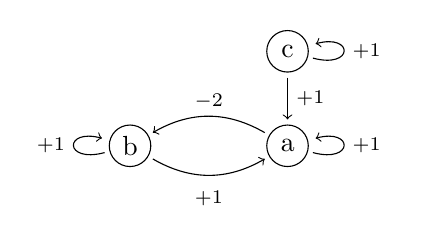
\begin{tikzpicture}[grn]
  \path[use as bounding box] (-1.3,-0.75) rectangle (3.5,1.5);
  \node[inner sep=0] (a) at (2,0) {a};
  \node[inner sep=0] (b) at (0,0) {b};
  \node[inner sep=0] (c) at (2,1.2) {c};
  \path[->]
    (b) edge[bend right] node[elabel, below=-2pt] {$+1$} (a)
    (c) edge node[elabel, right=-2pt] {$+1$} (a)
    (a) edge[bend right] node[elabel, above=-5pt] {$-2$} (b)
    (b) edge[in=-15+180, out=15+180, loop] node[elabel, left=-2pt] {+1} (b)
    (c) edge[in=15, out=-15, loop] node[elabel, right=-2pt] {+1} (c)
    (a) edge[in=15, out=-15, loop] node[elabel, right=-2pt] {+1} (a);
\end{tikzpicture}
}
\caption{\label{fig:BRN-inf1}
  Result of the IG inference performed on the PH of \pref{fig:runningPH-2}.
}
\end{figure}

\end{example}



\begin{example}
If we add the action $\PHfrappe{a_2}{b_0}{b_1}$ to the PH of \pref{fig:runningPH-2},
then two unsigned edges towards $b$ are inferred instead of the previous signed edges:
\begin{align*}
  E_+ &= \{\GRNedgef{b}{+}{1}{a}, \GRNedgef{c}{+}{1}{a}, \GRNedgef{a}{+}{1}{a}, \GRNedgef{c}{+}{1}{c}\}\\
  E_- &= \emptyset \qquad\qquad\qquad\qquad
  E_\uns = \{\GRNedgef{a}{\uns}{2}{b}, \GRNedgef{b}{\uns}{1}{b}\}
\end{align*}
This is due to the fact that the actions $\PHfrappe{a_2}{b_1}{b_0}$ and $\PHfrappe{a_2}{b_0}{b_1}$
introduce an oscillation only caused by $a$, which cannot be represented in Thomas modeling.
\end{example}

\section{Parametrization inference}\label{sec:infer-K}

Given the IG inferred from a PH as presented in the previous section, one can find the discrete parameters that model the behavior of the studied PH using the method presented in the following.
It relies on an exhaustive enumeration of all predecessors of each component in order to find attractor processes and returns a possibly incomplete parametrization, given the exhaustiveness of the cooperations.
The last step consists of the enumeration of all compatible complete parametrizations given this
set of inferred parameters, the PH dynamics and some biological constraints on parameters.

\subsection{Parameters inference}

This subsection presents some results related to the inference of independent discrete parameters from a given PH.
These results are equivalent to those presented in \cite{PMR10-TCSB}, with notation adapted to be shared with the previous section.
In addition, we introduce the well-formed PH for parameter inference property (\pref{pro:wf-ph-K}),
which implies that the inferred IG does not contain any unsigned interactions, and thus can be seen as the
regular IG $(\Gamma, E)$,
and that any processes in $\levels{b}{a}$ (resp. $\ulevels{b}{a}$) share the same behavior
regarding $a$.

\begin{property}[Well-formed PH for parameter inference]\label{pro:wf-ph-K}
A PH is well-formed for parameter inference if and only if
it is well-formed for IG inference, and
the IG $(\Gamma, E)$ inferred by \pref{pps:inference-IG}
verifies the following property:
\begin{align*}
  \begin{split}
  \forall a \in \Gamma, \forall b\in \GRNreg{a}&,
          \forall (i,j\in\levels{b}{a} \vee i,j\in\ulevels{b}{a}), \\
  & \quad \forall c \in \Gamma, ( (b\neq a\wedge c=a) \vee (c\in\PHpredec{a} \wedge b\in\PHdirectpredec{c})), \\
  & \qquad
                          \PHfrappe{b_i}{c_k}{c_l}\in\PHa \Leftrightarrow
                                  \PHfrappe{b_j}{c_k}{c_l}\in\PHa
  \end{split}
\end{align*}
\end{property}

Let $K_{a,\omega}$ be the parameter we want to infer for a given component $a \in \Gamma$
and $\omega \subset \GRNreg{a}$ a set of its regulators.
This inference, as for the IG inference, relies on the search of focal processes of the component for the given configuration of its regulators.

For each sort $b \in \GRNreg{a}$, we define a context $C^b_{a,\omega}$ in \pref{eq:param_context} that contains all processes representing the influence of the resources in the configuration modeled by $\omega$.
The context of a cooperative sort $\upsilon$ that regulates $a$ is given in
\pref{eq:param_context_coop} as the set of focal processes matching the current configuration.
$C_{a,\omega}$ refers to the union of all these contexts (\pref{eq:K-ctx}).
\begin{align}
  \label{eq:param_context}
  \forall b\in\Gamma,~
  C_{a,\omega}^b & \DEF \begin{cases}
    \levels{b}{a} & \text{if $b \in \omega$,}\\
    \ulevels{b}{a} & \text{if $b \notin \omega$,}\\
    L_b            & \text{otherwise;}\\
  \end{cases}
  \\
  \label{eq:param_context_coop}
  \forall \upsilon \in \PHpredec{a}\setminus\Gamma,~
  C_{a,\omega}^\upsilon & \DEF \{
  \upsilon(\sigma) \mid \sigma \in \textstyle\prod_{c\in\PHdirectpredec{\upsilon}}C_{a,\omega}^c \}
  \\
  C_{a,\omega} & \DEF \textstyle\bigcup_{b\in\PHpredec{a}} C^b_{a,\omega}
  \label{eq:K-ctx}
\end{align}

The parameter $K_{a,\omega}$ specifies to which values $a$ eventually evolves as long as the context
$C_{a,\omega}$ holds, which is precisely the definition of the $\focals$ function
(\pref{def:focals} in \pref{ssec:focal}),
where the focals reachability property can be derived from \pref{pro:wf-ph-K} and
\pref{eq:param_context_coop}.
Hence $K_{a,\omega} = \focals(a,C^a_{a,\omega},C_{a,\omega})$ if this latter is a non-empty interval
(\pref{pps:param_K}).

\begin{proposition}[Parameter inference]
\label{pps:param_K}
Let $(\PHs, \PHl, \PHh)$ be a Process Hitting well-formed for parameter inference, and $\IG = (\Gamma, E)$ the inferred IG.
Let $A$ (resp. $B$) $\subseteq \Gamma$ be the set of regulators that activate (resp. inhibit) a sort
$a$.
If $\focals(a,C^a_{a,\omega},C_{a,\omega})=\segm{a_i}{a_j}$ is a non-empty interval, then $K_{a,\omega} = \segm{i}{j}$.
\end{proposition}

\begin{example}
\label{ex:infer-param-runningPH-1}
Applied to the PH in \pref{fig:runningPH-1}, we obtain, in particular,
$K_{b,\emptyset} = \segm{0}{1}$ and
$K_{a,\{b,c\}} = \segm{2}{2}$,
while $K_{a,\{b\}}$ and $K_{a,\{c\}}$ can not be inferred.
\end{example}

\begin{example}
Regarding the PH in \pref{fig:runningPH-2}, we obtain
$K_{b,\emptyset} = \segm{0}{1}$,
$K_{a,\{b,c\}} = \segm{2}{2}$,
$K_{a,\{b\}} = \segm{1}{1}$,
and $K_{a,\{c\}} = \segm{1}{1}$.
For this PH, all parameters can be inferred, and the obtained parametrization is the one of \pref{fig:runningBRN}(right).
\end{example}

Given the \pref{pps:param_K}, we see that in some cases, the inference of the targeted parameter is impossible.
This can be due to a lack of cooperation between regulators: when two regulators independently hit a component, their actions can have opposite effects, leading to either an indeterministic evolution or to oscillations.
Such an indeterminism is not possible in a BRN as in a given configuration of regulators, a component can only have an interval attractor, and eventually reaches a steady-state.
In order to avoid such inconclusive cases, one has to ensure that no such behavior is allowed by
either removing undesired actions or using cooperative sorts to prevent opposite influences between
regulators.

\subsection{Admissible parametrizations}\label{ssec:admissible-K}

When building a BRN, one has to find the parametrization that best describes the desired behavior of the studied system.
Complexity is inherent to this process as the number of possible parametrizations for a given IG is exponential w.r.t. the number of components.
However, the method of parameters inference presented in this section gives some information about necessary parameters given a certain dynamics described by a PH.
This information thus drops the number of possible parametrizations, allowing to find the desired behavior more easily.

We first delimit the validity of a parameter (\pref{pro:K-valid}) in order to ensure that any
transition in the resulting BRN is allowed by the studied PH.
This is verified by the existence of a hit making the concerned component bounce into the direction
of the value of the parameter in the matching context.
Thus, assuming \pref{pro:wf-ph-K} holds, any transition in the inferred BRN corresponds to at least
one transition in the PH, proving the correctness of our inference.
We remark that any parameter inferred by \pref{pps:param_K} satisfies this property.

\begin{property}[Parameter validity]\label{pro:K-valid}
A parameter $K_{a,\omega}$ is valid w.r.t. the PH if and only if the following equation is verified:
\begin{align*}
  \forall a_i\in C^a_{a,\omega}, a_i \notin K_{a,\omega} \Longrightarrow
    (& \exists \PHfrappe{c_k}{a_i}{a_j}\in\PHa, c_k \in C^c_{a,\omega} \\
     & \wedge a_i < K_{a,\omega} \Rightarrow j > i \wedge  a_i > K_{a,\omega} \Rightarrow j <i )
\end{align*}
\end{property}

Then, we use some additional biological constraints on Thomas' parameters given in
\cite{BernotSemBRN}, that we sum up in the following three properties:

\begin{property}[Extreme values assumption]
Let $\IG = (\Gamma, E)$ be an IG. A parametrization $K$ on $\IG$ satisfies the \emph{extreme values assumption} if and only if:
\label{pro:param_enum_extreme}
\begin{align*}
  \forall b \in \Gamma, \GRNreg{b} \neq \emptyset \Longrightarrow \exists \omega \subset \GRNreg{b}, 0 \in K_{b,\omega} \wedge \exists \omega' \subset \GRNreg{b}, l_b \in K_{b,\omega'}
\end{align*}
\end{property}

\begin{property}[Activity assumption]
\label{pro:param_enum_activity}
Let $\IG = (\Gamma, E)$ be an IG. A parametrization $K$ on $\IG$ satisfies the \emph{activity assumption} if and only if:
\begin{align*}
  \forall b \in \Gamma, \forall a \in \GRNreg{b}, \exists \omega \subset \GRNreg{b}, K_{b,\omega} \neq K_{b,\omega \cup \{ a \}}
\end{align*}
\end{property}

\begin{property}[Monotonicity assumption]
\label{pro:param_enum_monotonicity}
Let $\IG = (\Gamma, E)$ be an IG. A parametrization $K$ on $\IG$ satisfies the \emph{monotonicity assumption} if and only if:
\begin{align*}
  \forall b \in \Gamma,
  \forall A^+ \subset \{ a \in \Gamma \mid \GRNedge{a}{+}{t}{b} \in E_+ \}&,
  \forall A^- \subset \{ a \in \Gamma \mid \GRNedge{a}{-}{t}{b} \in E_- \},\\
  K_{b,\omega \cup A^-} & \leqsegm K_{b,\omega \cup A^+}
\end{align*}
\end{property}

\section{Examples}\label{sec:examples}

This section details the implementation and usage of the piece of software developed for this work.
\pref{ssec:appli} gives a practical and detailed application of our results on a biological model taken from the literature,
while \pref{ssec:cpu} gives data related to the results and computation times of our software when applied to several large biological models.

\medskip

The inference methods described in this paper have been implemented as part of
\textsc{Pint}\footnote{Available at \url{http://process.hitting.free.fr}}, which gathers PH related tools.
Our implementation mainly consists in ASP programs that are solved using
Clingo\footnote{Available at \url{http://potassco.sourceforge.net}}.
The IG and parameters inference can be performed using the following command:\\
  \hspace*{1.2em}\texttt{ph2thomas -i model.ph -{}-dot ig.dot}\\
where \texttt{model.ph} is the PH model in \textsc{Pint} format,
and \texttt{ig.dot} is an output of the inferred IG in DOT format.
The (possibly partial) inferred parametrization will be returned on the standard output.
The admissible parametrizations enumeration is performed when adding the \texttt{-{}-full-enumerate} parameter to the command,
or \texttt{-{}-enumerate} instead to obtain only simple parameters (intervals of cardinality $1$).



\subsection{Biological application}\label{ssec:appli}

This subsection focuses on the study of the epidermal growth factor (EGF) receptor model detailed in~\cite{Sahin09}.
This model is represented by an IG containing 20 components and 52 edges.
A protein named EGF, having no regulator, can be considered as the only input,
and a chain of reactions leads to the activation of protein pRB which is responsible for regulating the cell division,
therefore making it essential to prevent cancer development.

Three models are created from the original IG, with different levels of precision regarding the cooperation between components.
The translation from an IG into a Process Hitting is not detailed here as it was previously covered in~\cite{PMR10-TCSB}.
Model (1) represents a translation of the raw IG into Process Hitting, that is,
without any knowledge of the Boolean rules (and therefore the cooperations) of the components.
Model (2) implements some of the rules based on the results of several knockdown experiments.
Model (3) is the totally refined model with all cooperations implemented given the Boolean functions of all components.
Therefore, those three models can be considered as successive refinements of the original and most general one.
The results of the IG and parameters inferences are detailed in \pref{tb:egfr20}
and discussed in the following alongside with details about their construction.

\begin{table}[ht]
~\hfill%\begin{center}
  \begin{tabular}{r|l|l|m{2cm}|m{2.5cm}|m{1.5cm}}
    \textbf{Model} & $\mathbf{|E|}$ & $\mathbf{|K|}$ & \textbf{Inferred parameters} & \textbf{Possible\newline models} & \textbf{Fixed points}
  \\\hline\hline
    (1) & $52$ & $196$ & $20$ & $2^{176}\simeq 9.6\cdot10^{52}$ & $0$   % v1_0.ph
  \\\hline
    (2) & $51$ & $192$ & $98$ & $2^{94}\simeq 2.0\cdot10^{28}$ & $0$    % v2_1.ph
  \\\hline
    (3) & $51$ & $192$ & $192$ & $1$ & $3$                              % ori.ph
  \\\hline
  \end{tabular}
\hfill~%\end{center}
  \caption{%
  Results of the IG and parameters inference on three models
  derived from the EGF receptor model of~\cite{Sahin09}
  with different precisions in the definition of the cooperations.
  Model (1) contains no cooperations between the components.
  Several cooperations were included in model (2) under the form of 14 cooperative sorts
  and all of them were included in Model (3) under the form of 22 cooperative sorts.
%  Model (3) models all the Boolean functions between components using 22 cooperative sorts.
  The second column gives the number of edges in the IG inferred with \pref{pps:inference-IG}
  (the number of nodes is always the number of components in the model, that is, 20).
  The third column gives the number of parameters in the model (given the IG),
  the fourth column gives the number of parameters that could be inferred using \pref{pps:param_K},
  and the fifth column consequently gives the number fo compatible models with the studied PH model,
  which exponentially depends on the number of parameters that could not be inferred.
  Finally, the last column gives the number of fixed points in the PH model,
  computed with another existing PH tool included in \textsc{Pint}.
  }
  \label{tb:egfr20}
\end{table}

Model (1) encompasses only sole interactions between components, that is,
independent activations or inhibitions of a component on another given the regulations specified in the original IG.
Therefore, the IG inferred from model (1) is the same as the IG used to create the model,
with one additional positive auto-edge on the only input EGF (which is due to its absence of regulators).
The only parameters that could be inferred are the parameters for the extreme cases
(all activators present and all inhibitors absent, and the reverse).
This first model therefore abstracts a large number of Thomas models as a lot of parameters are left undecided.

In order to build model (2), 14 cooperative sorts were added in order to model the Boolean functions of several components
(consisting of AND and OR operands).
To do so, the following components were noticed due to their importance in the chain of reactions:
CDK4, CDK6, CycD1, ER$\alpha$ and c-MYC.
Indeed, knockdown experiments have been conducted in~\cite{Sahin09}
and the results showed that knocking down these components lead to an important decrease in the production of pRB.
We therefore concluded that these components were involved in other components' Boolean functions
in a way that the knockdown of the former was sufficient to prevent the production of the latter (which is typical of AND operands).
In order to reproduce such requirements, the Boolean functions of their successors,
that is CDK4, CDK6, prB, p21, p27, IGF1R, MYC, CycD1 and CycE1,
were modeled as cooperative sorts, if needed.
In theory, 9 cooperative sorts would have sufficed, but the chaining of cooperative sorts described
in \pref{ssec:PH} was used to reduce the number of processes in each cooperative sort.
We note that the added cooperations allowed to infer about half the parameters.
However, the number of possible Thomas models that can be inferred from this PH is still significant
because of the numerous remaining unknown parameters.
Furthermore, the inferred IG contains one edge less than the original IG. This is due to the fact that
one of the Boolean functions could in fact be simplified in a way that this component did not appear anymore.
No edge have therefore been inferred by our method in this case.

Finally, model (3) was build using all the Boolean functions provided in~\cite{Sahin09}.
These functions take the form of 22 cooperative sorts into the model in order to match the desired behavior of the system.
As all cooperations are fully defined in this model, all the parameters are inferred and only one Thomas model can be derived.
We note also that this PH model is the only one containing at least one fixed point,
which indicates the possibility of a steady state once the input signal is completely propagated.



\subsection{Computation times on several large models}\label{ssec:cpu}

The current implementation can successfully handle large PH models of BRNs found in the literature such as:
\begin{itemize}
  \item the EGF receptor model from~\cite{Sahin09} with 20 components presented in the last subsection,
  \item a T cell receptor model described as an IG in~\cite{Klamt06}, which contains 40 components and 14 cooperative
    sorts\footnote{All models mentioned in this section are available as examples distributed with \textsc{Pint}.}.
\end{itemize}
For each model, IG and parameters inferences are performed together in less than a second
on a standard desktop computer.

Bigger models related to the aforementioned systems were also tested with our implementation:
\begin{itemize}
  \item a model of the T cell receptor with 94 components, described in~\cite{SaezRodriguez2007},
  \item a model of the EGF receptor with 104 components, described in~\cite{Samaga2009}.
\end{itemize}
These two models were obtained in a previous work by an automatic translation from CellNetAnalyzer~\cite{klamt2007structural} formalism.

The composition of all models and the results of the inferences are summarized in \pref{tb:computation}.
We note that due to a very high number of parameters, no parameters inference could be performed on the $94$ and $104$ component models.
These models would therefore be more efficiently studied as PH than as BRNs.
Finally, we note that the complexity of the method is exponential in the number of regulators of one
component and linear in the number of components.

\begin{table}[ht]
\begin{center}
  \begin{tabular}{r|c|c|c|c|c}
    \textbf{Model} & $\mathbf{|\Gamma|}$ & $\mathbf{|\PHs \setminus \Gamma|}$ & \textbf{$\Delta t$ IG} & \textbf{$\Delta t$ K} & $\mathbf{|K|}$
\\\hline\hline
    EGF receptor \cite{Sahin09} & $20$ & $22$ & <1s & <1s & 192
\\\hline
    T cell receptor \cite{Klamt06} & $40$ & $14$ & <1s & <1s & 143
\\\hline
    T cell receptor \cite{SaezRodriguez2007} & $94$ & $39$ & 10s & --- & $2.1\cdot10^{9}$
\\\hline
    EGF receptor \cite{Samaga2009} & $104$ & $89$ & 3min 20s & --- & $4.2\cdot10^{6}$
  \end{tabular}
\end{center}
\caption{%
  Computation times and several pieces of information related to the IG and parametrization inferences of four biological models.
  The second column gives the number of components of each model and
  the third column gives the number of cooperative sorts used to model joint actions.
  The fourth (resp.~fifth) column gives the computation times of the IG inference (resp.~the parametrization inference).
  The last column gives the number of parameters in each model.
  Due to the too high number of parameters, parametrization inference could not be performed on the $94$ and $104$ component models.
  }
\label{tb:computation}
\end{table}

\section{Conclusion and Discussion}

This work establishes the abstraction relationship between PH and Thomas' approaches for
qualitative BRN modeling.
The PH allows an abstract representation of BRNs dynamics (allowing incomplete knowledge on the
cooperation between components) that cannot be exactly represented in Ren\'e Thomas' formalism by a
single instance of BRN parametrization.
This motivates the concretization of PH models into a set of compatible Thomas' models in order to benefit
of the complementary advantages of these two formal frameworks.

We first propose an original inference of the Interaction Graph (IG) from a BRN
having its dynamics specified in the PH framework.
An IG gives a compact abstract representation of the influence of the components between each
others.
Then, based on a prior inference of Ren\'e Thomas' parametrization for BRNs from a PH model, we
delimit the set of compatible Thomas' parametrizations that are compatible with the PH dynamics,
and give arguments for their correctness.
A parametrization is compatible with the PH if its dynamics (in terms of possible transitions) is included in the PH dynamics.
The enumeration of such parametrizations is efficiently tackled using Answer Set Programming.
We illustrated the overall method with several results on large biological models.

Several extensions of the presented work are now to be considered.
First, further work on the inference of the IG would lead to better understand and possibly avoid
the presence of some of the current spurious auto-edges.
Second, the inference of BRN multiplexes \cite{BernotMultiplexes} may be of practical interest 
as they allow to implicitly reduce the possible parametrizations by making cooperations appear
in the IG.
Because of its atomicity, the PH allows to specify a range of cooperations that cannot be
completely captured by a single instance of BRN multiplexes, then encouraging the inference of a set
of compatible ones.
Finally, in order to improve the performances in the IG inference, we will consider projection operations on
the PH structure to undo cooperations between components and reduce the cardinality of
configurations to explore by making the interactions independent.

\paragraph{Acknowledgement}
This work was partially supported by the Fondation Centrale Initiatives and
the French National Agency for Research (ANR-10-BLANC-0218 BioTempo project).
The work of LP was supported by the Swiss SystemsX.ch project.


\bibliographystyle{elsarticle-num}
\bibliography{biblio}

%\input{parts/contributions}

\end{document}
